% Include preamble
\documentclass[12pt,a4paper]{article}
\usepackage[french,english]{babel}
\usepackage[T1, T2A]{fontenc}
% Load Package
% a third test
% a 5 test
\usepackage[margin=1in]{geometry} % for margin
\usepackage{blindtext}
\usepackage{graphicx}
\usepackage{multicol}
\usepackage{tabularx}
\usepackage{booktabs}
\usepackage{pgffor}
\usepackage{color}
\usepackage[hyperfootnotes=true,colorlinks=true,allcolors={blue}]{hyperref}
\usepackage{ifthen}
\usepackage{indentfirst}
\usepackage{dcolumn}

\usepackage{nameref}
\usepackage{placeins} % put this in your pre-amble
\usepackage{flafter}  % put this in your pre-amble
\usepackage{float} % to manage figure float
\usepackage{authblk} % for co-author
\usepackage{pdfpages}
\usepackage{listings} % for formating code
\usepackage{dirtytalk} % for inserting quotation
% Control footnotes spacing
%\usepackage{footnote}
%\usepackage[multiple]{footmisc}
\setlength{\footnotesep}{0.3cm}%
\setlength{\skip\footins}{0.7cm}

\usepackage{bookmark}
%\usepackage{lmodern}
%\usepackage{mathptmx} % for nice font
\fontfamily{cmss}

\hypersetup{
  colorlinks=true,
  allcolors=blue
}

\usepackage{threeparttable}
\usepackage{booktabs, longtable}
\usepackage{tabularx}
\usepackage[singlelinecheck=false]{caption}
% for source under image
\newcommand{\source}[1]{\caption*{Source: {#1}} }

% set space interligne etc
\usepackage{setspace}
\onehalfspacing




%\usepackage{amssymb} %maths
%\usepackage{amsmath} %maths
\usepackage{siunitx} % using plus-minus instead of std
\usepackage[utf8]{inputenc} %useful to type directly diacritic characters
\usepackage[autostyle]{csquotes}
\DeclareUnicodeCharacter{2212}{-} % Unicode U+2212 is MINUS SIGN, which is not set up by default with inputenc
\DeclareUnicodeCharacter{2009}{~} % Unicode U+2212 is MINUS SIGN, which is not set up by default with inputenc{00A0}{~}

\DeclareUnicodeCharacter{0080}{+} % Unicode U+2212 is MINUS SIGN, which is not set up by default with inputenc{00A0}{~}

\DeclareUnicodeCharacter{0301}{-} % Unicode U+2212 is MINUS SIGN, which is not set up by default with inputenc{00A0}{~}

\DeclareUnicodeCharacter{0300}{-} % Unicode U+2212 is MINUS SIGN, which is not set up by default with inputenc{00A0}{~}

\DeclareUnicodeCharacter{001B}{-} % Unicode U+2212 is MINUS SIGN, which is not set up by default with inputenc{00A0}{~}

% Count of words
\usepackage{moreverb} % for verbatim ouput
\immediate\write18{texcount  -inc -merge -nobib -sum -sub=section \jobname.tex > ./texcount.tex}
\newcommand\wordcount{\verbatiminput{./texcount.tex}}

% Include csv files

% normal header stat here
\title{Fiscal Impact of Immigration in Canada: A National Transfer Accounting Approach}
\author[1]{Gilbert MONTCHO}
\author[3]{Julien Navaux}
\author[1]{Yves CARRIERE}
\author[2]{Marcel MERETTE}

\affil[1]{Department of Demography, University of Montreal}
\affil[2]{Department of Economics, University of Ottawa}
\affil[3]{Research Chair in Intergenerational Economics}

%\affil[3]{Chaire de recherche sur les enjeux �conomiques interg�n�rationnels}

\date{}


\begin{document}
% remove extra space btw table caption and table
%\captionsetup[table]{skip=0pt}
% Hide the default abstract title
%\renewcommand{\abstractname}{\vspace{-\baselineskip}}
\maketitle
\begin{abstract}
 Population aging has become the intersection of heated debates in advanced economies and one of the fierce is the role of immigration not only as a source of additional labour supply but also as a possible solution to alleviate the pressure on public finances. While the impact of immigration on various aspects of the labour market has been extensively researched, its fiscal impact on public finances has received less attention. In this study, we apply the National Transfer Account(NTA) and Demographic Analysis methods to estimate the net fiscal cost for immigrants and natives in Canada between 1997 and 2016. Results show that even though immigrants arrive in Canada with education and skill earned at the expense of their home country, the average immigrant has cost to the state about 3590\$ (2015 price) more than the average natives, per year between 1997 and 2016.

\end{abstract}

 \section*{Background}\label{sec:into}

 In the 2008 European Social Survey, 44\% of European citizens believed that immigrants receive more than they contribute, with only 15\% believing that they receive less \citep{Dustmann:2014dr}. While some empirical studies \citep{Fehr:2003gq,Chojnicki:2011vu,Borjas:2014hr} tend to support this view, many are those who believe that skilled immigrants make a large fiscal contribution \citep{Akin:2012gh,Storesletten:2000cn,Dustmann:2014dr} and even unskilled immigrants may be net contributors if they eventually depart or make few claims on government expenditure while in the country \citep{Rowthorn:2008kk}. As a result, immigrant intake has been increasing in most developed countries \citep{Card:2016ku} and the immigration debate has become hotter than never before. In Canada for instance, results from \citet{Ileri:2019hf,Dungan:2013jp,Hering.Klassen.2010}, support positive effect of immigration on public finance while \citet{Grubel:2012wo,Javdani:2013gu,Akbari:1989fh} found negative effect.

 \vspace{0.7em}\par
 This apparent conflict is partially due to the use of different immigrant populations and assumptions about the consumption of public goods \citep{Grubel:2012wo}. Furthermore, most studies consider only transfers to and from the state that are directly related to the individual, while transfers through the family are left out \citep{dAlbis:2019de}. In this study, we use the National Transfer Account (NTA) method which takes an intergenerational approach and allows us to account for costs and contributions that involve both the family and the state, over a relatively large number of cohorts \citep{Mason:2011wc,UnitedNations:2013vz}.

 \section*{Methods \& Data Sources}\label{sec:data}
 The NTA method introduced age into the System of National Accounts(SNA) by disaggregating national income, consumption, and savings by age and therefore to take into account intergenerational transfers made through the State or the family. This article goes further by splitting transfer to and from the state by immigration status. Then it applies the resulting cost-contribution profile to mortality and census data to account for changes in life expectancy and immigrant arrival age. Cost-contribution profiles are constructed with data from Canadian Economic Accounts, Consumers Surveys and Population estimate especially tailored by Statistics Canada for the study. Surveys data include the Survey of labour and Income Dynamics (SLID) from 1997 to 2011, the Canadian Income Survey (CIS) from 2011 to 2016 and the Survey of Household Spending (SHS) from 1997 to 2016.

 \section*{Preliminary results}\label{sec:result}
 Annual cost-contribution (cost minus contributions) profiles constructed with the NTA show that between 1997 and 2015 and in 2015 Price, the average native makes a net contribution of about 120\$ per year while the average immigrant induced a net cost of 1590\$ per year (\autoref{fig:TxSum}: A). These results are obtained by dividing the aggregated cost-contribution by the total population and then averaging over the 19 years of the study. To account for the difference in age structure by immigration status, we standardize the age profiles with the age structure of the entire population. This leads to an increase in net contributions of 660\$ for a native and net costs of about 2930\$ for an immigrant (\autoref{fig:TxSum}: B). \autoref{fig:txAge9715} show the age profiles of cost-contribution for 1997 and 2015 as examples. Compatible with the life cycle theories of consumption, cost-contributions are positive at younger and older ages but negative during prime age as production surpasses consumption.

 \vspace{0.7em}\par
 To sum up, at equal age, the average immigrant has cost to the state about 3590\$ per year, more than the average natives, between 1997 and 2016. These results may stand against expectations of a positive impact of immigration on public finances, especially for recent immigrants for whom economic factors have motivated the admission.

 \vspace{0.7em}\par
 As most immigrants arrive in Canada after they have become a labour force participant, immigration is expected to be a saving to taxpayers as they do not have to pay for the costs of child care and education before immigrants arrive; For example, \citet{Dustmann:2014dr} found that between 1995 and 2011 European and non-European immigrants endowed the UK labour market with human capital that would have cost £14 and £35 billion respectively if it were produced through the British education system. Added this to the fact that somImmigrantsts will return to their home country to spend the last part of their life that is most cost-intensive in health care \citep{Bratsberg:2014cl}, it would be reasonable to expect a net contribution froImmigrantsts to the public purse. Therefore, further investigations will analyze how the age at immigration affects the cost-contribution oImmigrantsts comparednativeveses for various cohorts and over the lifecycle.


 \begin{figure}[H]%
 \caption{Cost-contribution per Capita for native and Immmigrants between 1997 and 2015}
 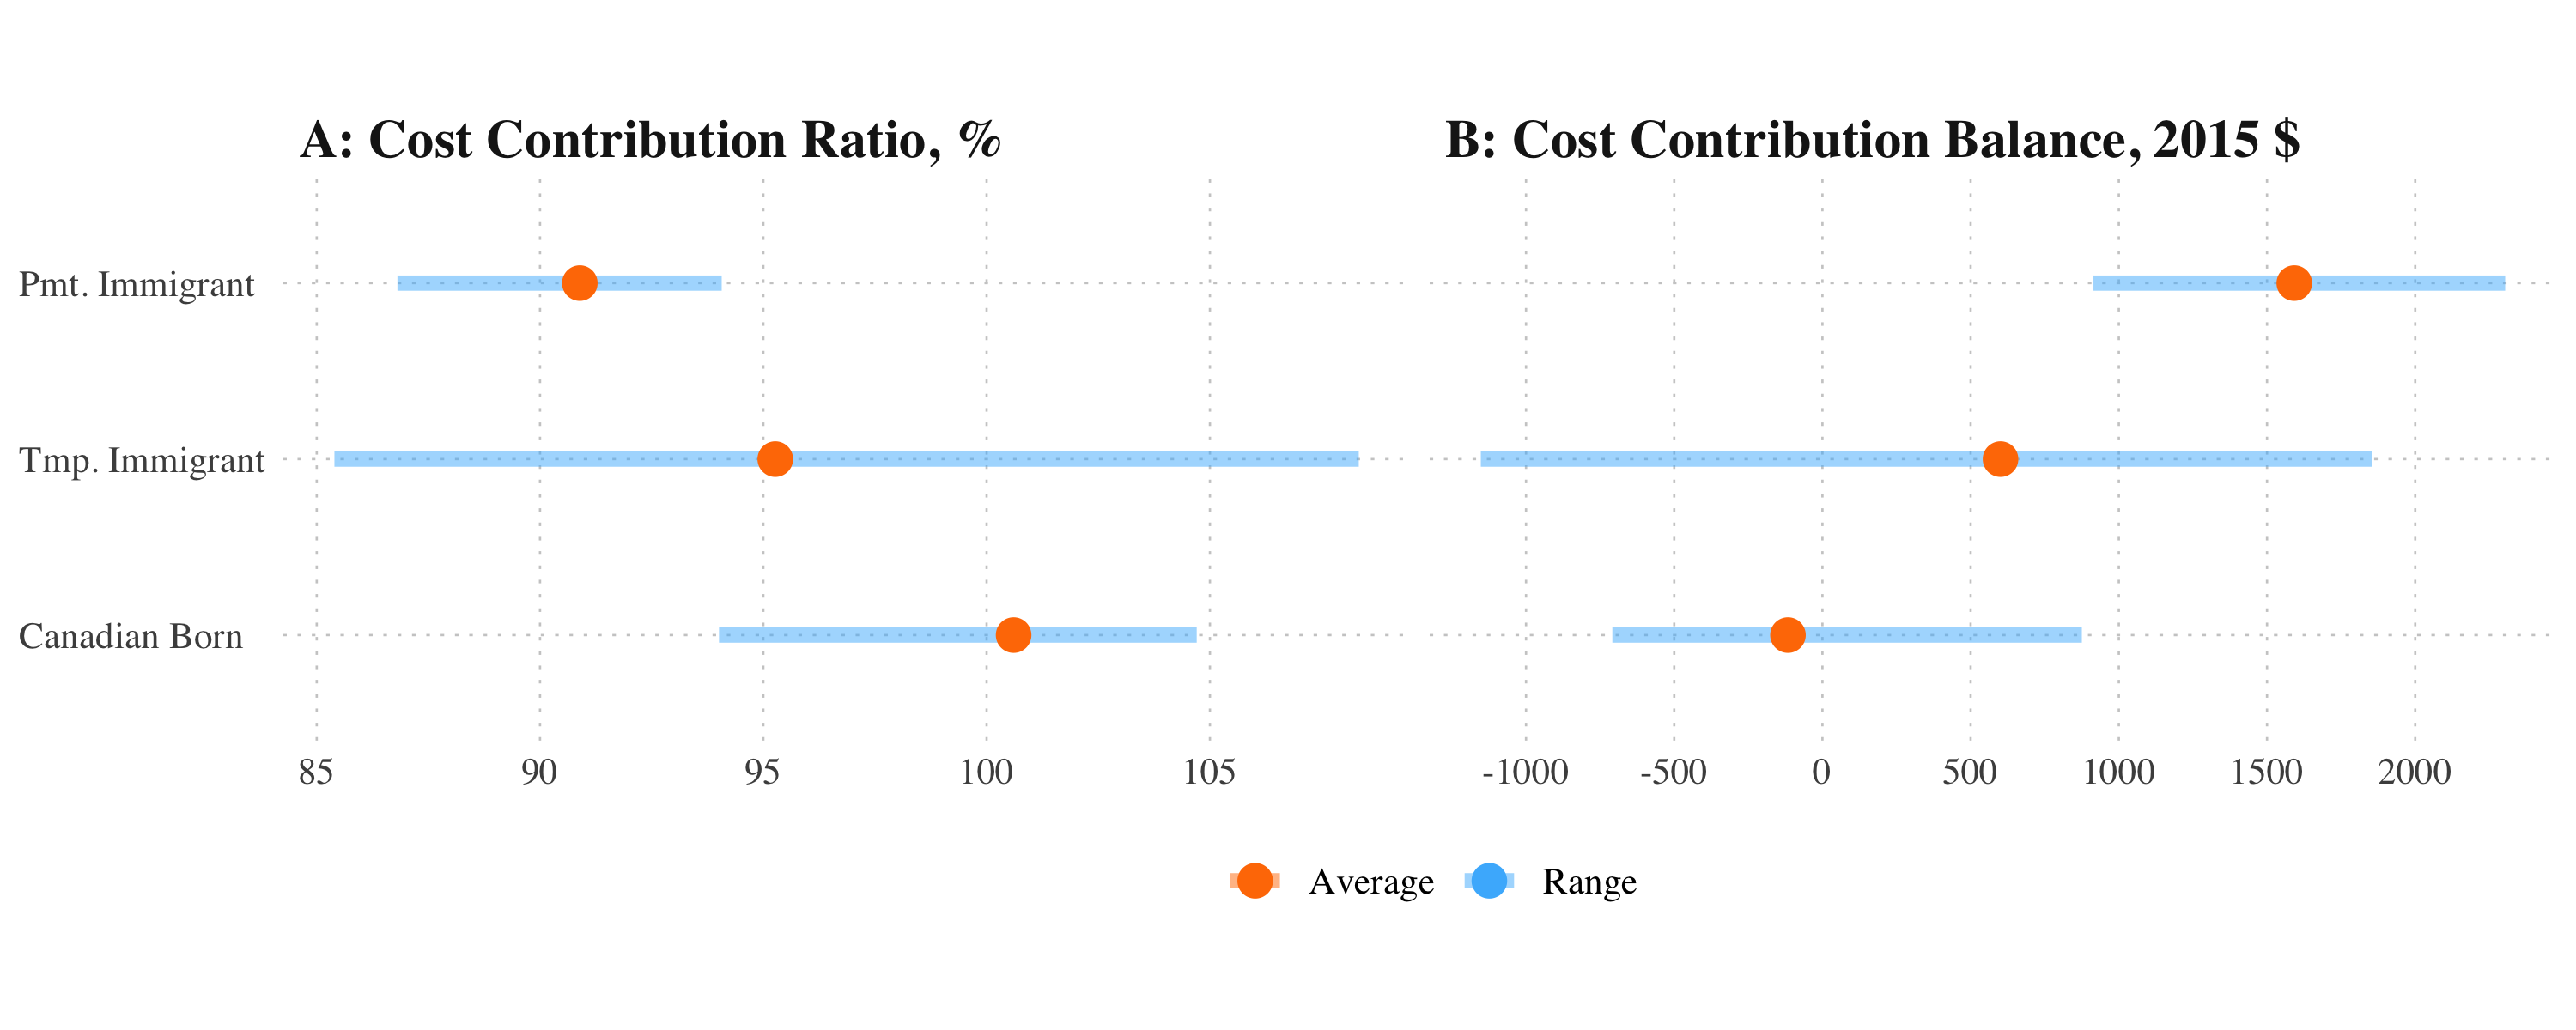
\includegraphics[width=1\textwidth]{./res/TxSum.pdf}%
 \label{fig:TxSum}%
\end{figure}%



 \begin{figure}[H]%
 \caption{ Cost-contribution profile for native and Immmigrants for 1997 and 2015}
 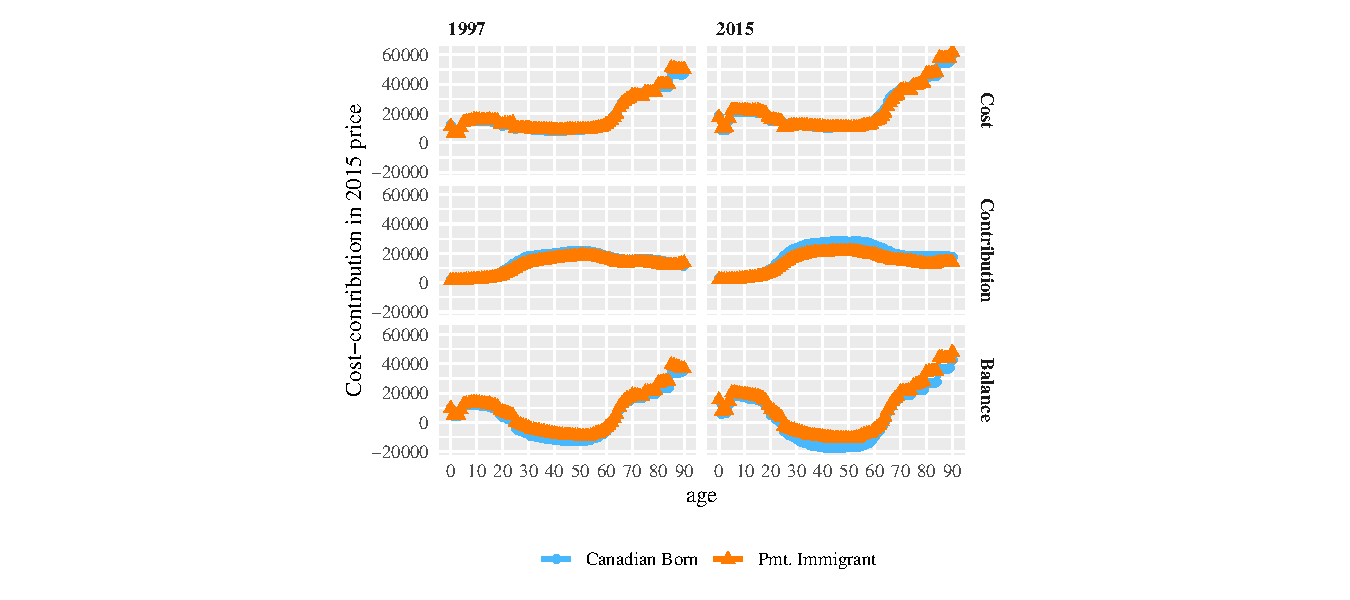
\includegraphics[width=1\textwidth]{./res/txAge9715.pdf}%
 \label{fig:txAge9715}%
\end{figure}%


 \newpage
 \section*{References}
 \printbibliography[heading=none]

\end{document}